\section*{Exercise 2 - Transformation methods}

\subsection*{Question 1: Independence and Distributions of R and S}

\textbf{Given:} $X_1 \sim \text{Gamma}(a,1)$ and $X_2 \sim \text{Gamma}(b,1)$ are independent.
\\[2mm]
\textbf{To prove:} $R = \frac{X_1}{X_1 + X_2}$ and $S = X_1 + X_2$ are independent, with $R \sim \text{Beta}(a,b)$ and $S \sim \text{Gamma}(a+b,1)$.

The joint density of $(X_1, X_2)$ is:
\begin{equation*}
f_{X_1,X_2}(x_1, x_2) = \frac{x_1^{a-1} x_2^{b-1} e^{-(x_1+x_2)}}{\Gamma(a)\Gamma(b)}
\end{equation*}

Using the transformation $R = \frac{X_1}{X_1 + X_2}$, $S = X_1 + X_2$:
\begin{align*}
X_1 &= RS \\
X_2 &= S(1-R)
\end{align*}

The Jacobian is:
\begin{equation*}
J = \begin{vmatrix}
s & r \\
-s & 1-r
\end{vmatrix} = s
\end{equation*}

The joint density of $(R,S)$ becomes:
\begin{align*}
f_{R,S}(r,s) &= \frac{(rs)^{a-1} [s(1-r)]^{b-1} e^{-s}}{\Gamma(a)\Gamma(b)} \cdot s \\
&= \frac{s^{a+b-1} r^{a-1} (1-r)^{b-1} e^{-s}}{\Gamma(a)\Gamma(b)} \\
&= \left[\frac{\Gamma(a+b)}{\Gamma(a)\Gamma(b)} r^{a-1}(1-r)^{b-1}\right] \cdot \left[\frac{s^{a+b-1} e^{-s}}{\Gamma(a+b)}\right]
\end{align*}

This factors as $f_R(r) \cdot f_S(s)$, proving independence with $R \sim \text{Beta}(a,b)$ and $S \sim \text{Gamma}(a+b,1)$.

\subsection*{Question 2: Distribution of $X = U^{1/a}$}
\textbf{Given:} $U \sim \text{U}[0,1]$ and $a > 0$.
\\[2mm]
\textbf{To prove:} $X = U^{1/a} \sim \text{Beta}(a,1)$.

For $x \in (0,1)$:
\begin{equation*}
P(X \leq x) = P(U^{1/a} \leq x) = P(U \leq x^a) = x^a
\end{equation*}

The PDF is:
\begin{equation*}
f_X(x) = \frac{d}{dx}[x^a] = ax^{a-1}
\end{equation*}

This matches the $\text{Beta}(a,1)$ density: $\frac{\Gamma(a+1)}{\Gamma(a)\Gamma(1)} x^{a-1} = ax^{a-1}$.

\subsection*{Question 3: Conditional Distribution}

For $t \in (0,1)$, the event 
$${Y/(Y+Z) \leq t, Y+Z \leq 1}$$
is equivalent to 
$${(y,z): y \leq (t/(1-t)) z, y \leq 1-z, y>0, z>0}$$. 

Splitting at $z = 1 - t$ where $(t/(1-t)) z = 1 - z$:

$$
P(Y/(Y+Z) \leq t, Y+Z \leq 1)
= \int_{z=0}^{1-t} \int_{y=0}^{(t/(1-t)) z}   a(1-a) y^{a-1} z^{-a} dy dz
$$

$$
\int_{z=1-t}^{1} \int_{y=0}^{1-z} a(1-a) y^{a-1} z^{-a} dy dz = (1-a) t^a (1-t)^{1-a} + (1-a) \int_{0}^{t} w^a (1-w)^{-a} dw.
$$
In particular,
$$
P(Y+Z \leq 1) = P(Y/(Y+Z) \leq 1, Y+Z \leq 1) = a(1-a) \int_{0}^{1} w^{a-1} (1-w)^{-a} dw = a(1-a) B(a, 1-a).
$$

Differentiate the function of t above:
$d/dt P(Y/(Y+Z) \leq t, Y+Z \leq 1) = a(1-a) t^{a-1} (1-t)^{-a}$.

Therefore, the conditional density of $W = Y/(Y+Z)$ given $Y+Z \leq 1$ is
$$
f_{W|Y+Z\leq 1}(t) = [a(1-a) t^{a-1} (1-t)^{-a}] / [a(1-a) B(a, 1-a)]
= [1 / B(a, 1-a)] t^{a-1} (1-t)^{-a}, 0 < t < 1,
$$

which is the Beta(a, 1-a) density. Hence $W | (Y+Z \leq 1)\sim $ Beta(a, 1-a).

% \textbf{Given:} $U, V \sim \text{U}[0,1]$ independent, $Y = U^{1/a}$, $Z = V^{1/(1-a)}$ for $a \in (0,1)$.
% \\[2mm]
% \textbf{To show:} $W = \frac{Y}{Y+Z} \mid \{Y+Z \leq 1\} \sim \text{Beta}(a, 1-a)$.

% The constraints are:
% \begin{align*}
% \frac{Y}{Y+Z} &\leq t \Rightarrow Z \geq \frac{(1-t)Y}{t} \\
% Y + Z &\leq 1 \Rightarrow Z \leq 1-Y
% \end{align*}

% For compatibility: $Y \leq t$.
% \begin{equation*}
% P\left(\frac{Y}{Y+Z} \leq t, Y+Z \leq 1\right) = \int_0^t \int_{\frac{(1-t)y}{t}}^{1-y} ay^{a-1} \cdot (1-a)z^{-a} \, dz \, dy
% \end{equation*}

% After integration, this yields the conditional distribution:
% \begin{equation*}
% W \mid \{Y+Z \leq 1\} \sim \text{Beta}(a, 1-a)
% \end{equation*}

% \section*{Detailed Integration for Part 3: Conditional Distribution}
% \subsection*{Setup and Joint Density}
% Given: $U, V \sim \text{U}[0,1]$ independent, $a \in (0,1)$, $Y = U^{1/a}$, $Z = V^{1/(1-a)}$.
% From the transformations:
% \begin{align}
% Y &= U^{1/a} \Rightarrow U = Y^a \\
% Z &= V^{1/(1-a)} \Rightarrow V = Z^{1-a}
% \end{align}
% The joint density of $(Y,Z)$ is obtained using the Jacobian:
% \begin{align}
% \frac{\partial u}{\partial y} &= ay^{a-1}, \quad \frac{\partial v}{\partial z} = (1-a)z^{-a} \\
% f_{Y,Z}(y,z) &= f_{U,V}(y^a, z^{1-a}) \cdot ay^{a-1} \cdot (1-a)z^{-a} \\
% &= 1 \cdot ay^{a-1} \cdot (1-a)z^{-a} \\
% &= a(1-a)y^{a-1}z^{-a}
% \end{align}
% for $y, z \in (0,1)$.
% \subsection*{Setting up the Integration Region}
% We need to compute:
% $$P\left(\frac{Y}{Y+Z} \leq t, Y+Z \leq 1\right)$$
% The constraints are:
% \begin{align}
% \frac{Y}{Y+Z} &\leq t \Rightarrow Y \leq t(Y+Z) \Rightarrow Y \leq tZ/(1-t) \text{ (for } t < 1) \\
% Y + Z &\leq 1 \Rightarrow Z \leq 1-Y
% \end{align}
% Following the hint, we express both as constraints on $Z$:
% - From constraint 1: $Z \geq \frac{(1-t)Y}{t}$
% - From constraint 2: $Z \leq 1-Y$
% For these constraints to be compatible, we need:
% $$\frac{(1-t)Y}{t} \leq 1-Y$$
% $$\Rightarrow (1-t)Y \leq t(1-Y) \Rightarrow (1-t)Y \leq t - tY$$
% $$\Rightarrow Y(1-t+t) \leq t \Rightarrow Y \leq t$$
% \subsection*{Detailed Integration}
% The probability becomes:
% \begin{align}
% &P\left(\frac{Y}{Y+Z} \leq t, Y+Z \leq 1\right) \\
% &= \int_0^t \int_{\frac{(1-t)y}{t}}^{1-y} a(1-a)y^{a-1}z^{-a} \, dz \, dy
% \end{align}
% \textbf{Step 1: Inner integration with respect to $z$}
% \begin{align}
% \int_{\frac{(1-t)y}{t}}^{1-y} z^{-a} \, dz &= \left[\frac{z^{1-a}}{1-a}\right]_{\frac{(1-t)y}{t}}^{1-y} \\
% &= \frac{1}{1-a}\left[(1-y)^{1-a} - \left(\frac{(1-t)y}{t}\right)^{1-a}\right] \\
% &= \frac{1}{1-a}\left[(1-y)^{1-a} - \frac{(1-t)^{1-a}y^{1-a}}{t^{1-a}}\right]
% \end{align}
% \textbf{Step 2: Outer integration with respect to $y$}
% \begin{align}
% &P\left(\frac{Y}{Y+Z} \leq t, Y+Z \leq 1\right) \\
% &= a(1-a) \cdot \frac{1}{1-a} \int_0^t y^{a-1}\left[(1-y)^{1-a} - \frac{(1-t)^{1-a}y^{1-a}}{t^{1-a}}\right] dy \\
% &= a \int_0^t y^{a-1}(1-y)^{1-a} \, dy - a\frac{(1-t)^{1-a}}{t^{1-a}} \int_0^t y^{a-1+1-a} \, dy \\
% &= a \int_0^t y^{a-1}(1-y)^{1-a} \, dy - a\frac{(1-t)^{1-a}}{t^{1-a}} \int_0^t y^{0} \, dy \\
% &= a \int_0^t y^{a-1}(1-y)^{1-a} \, dy - a\frac{(1-t)^{1-a}}{t^{1-a}} \cdot t \\
% &= a \int_0^t y^{a-1}(1-y)^{1-a} \, dy - a(1-t)^{1-a}t^{a}
% \end{align}
% \textbf{Step 3: Evaluating the first integral using Beta function}
% The integral $\int_0^t y^{a-1}(1-y)^{1-a} \, dy$ is related to the incomplete Beta function.
% Using the substitution $u = y/t$, $du = dy/t$:
% \begin{align}
% \int_0^t y^{a-1}(1-y)^{1-a} \, dy &= t^a \int_0^1 u^{a-1}(1-tu)^{1-a} \, du
% \end{align}
% For the case where we need the complete result, we can show that:
% \begin{align}
% \int_0^t y^{a-1}(1-y)^{1-a} \, dy = t^a B(a, 1-a) - \int_t^1 y^{a-1}(1-y)^{1-a} \, dy
% \end{align}
% \textbf{Step 4: Final simplification}
% After careful algebraic manipulation (which involves several integration by parts and Beta function identities), the result simplifies to:
% \begin{align}
% P\left(\frac{Y}{Y+Z} \leq t, Y+Z \leq 1\right) &= P(Y+Z \leq 1) \cdot \frac{\Gamma(a+1-a)}{\Gamma(a)\Gamma(1-a)} \int_0^t w^{a-1}(1-w)^{(1-a)-1} \, dw \\
% &= P(Y+Z \leq 1) \cdot \frac{\Gamma(1)}{\Gamma(a)\Gamma(1-a)} \int_0^t w^{a-1}(1-w)^{-a} \, dw \\
% &= P(Y+Z \leq 1) \cdot \frac{1}{\Gamma(a)\Gamma(1-a)} \int_0^t w^{a-1}(1-w)^{(1-a)-1} \, dw
% \end{align}
% \textbf{Step 5: Conditional probability}
% Therefore:
% \begin{align}
% P\left(\frac{Y}{Y+Z} \leq t \mid Y+Z \leq 1\right) &= \frac{P\left(\frac{Y}{Y+Z} \leq t, Y+Z \leq 1\right)}{P(Y+Z \leq 1)} \\
% &= \frac{\Gamma(a+(1-a))}{\Gamma(a)\Gamma(1-a)} \int_0^t w^{a-1}(1-w)^{(1-a)-1} \, dw \\
% &= \frac{\Gamma(1)}{\Gamma(a)\Gamma(1-a)} \int_0^t w^{a-1}(1-w)^{(1-a)-1} \, dw
% \end{align}
% This is precisely the CDF of a $\text{Beta}(a, 1-a)$ distribution, proving that:
% $$W = \frac{Y}{Y+Z} \mid \{Y+Z \leq 1\} \sim \text{Beta}(a, 1-a)$$


\subsection*{Question 4}

\subsection*{Question 5}

This procedure implements \textbf{Johnk's algorithm} for generating $\text{Gamma}(a, 1)$ 
random variables when $a \in (0, 1)$. See page 418 in Non-Uniform Random Variate Generation
by L. Devroye, Springer-Verlag, 1986.

\textbf{Analysis of the algorithm:}
\begin{enumerate}
    \item Steps (a)-(c) generate $(Y, Z)$ conditional on $Y + Z \leq 1$ where:
   \begin{itemize}
    \item $Y = U^{1/a}$ and $Z = V^{1/(1-a)}$ for independent $U, V \sim \mathcal{U}[0,1]$
    \item From Question 3, we know that $W = \frac{Y}{Y+Z} \mid Y+Z \leq 1 \sim \text{Beta}(a,1-a)$
    \end{itemize}
    \item Step (d) generates $T \sim \text{Exp}(1) = \text{Gamma}(1,1)$ since:

 $$T = -\log(A) \sim \text{Exp}(1) \text{ when } A \sim \mathcal{U}[0,1]$$
\item Step (e) returns $TW = T \cdot \frac{Y}{Y+Z}$, which from Question 4 has distribution:

 $$TW \mid Y+Z \leq 1 \sim \text{Gamma}(a, 1)$$
\end{enumerate}

\textbf{Relevance for simulations:}
This algorithm is particularly useful because:
\begin{itemize}
    \item It generates $\text{Gamma}(a,1)$ for $a \in (0,1)$, which cannot be done by summing exponentials
    \item It only requires uniform random variables
    \item The acceptance probability is $\frac{1}{B(a,1-a)} = \frac{\Gamma(a)\Gamma(1-a)}{\Gamma(1)} = \Gamma(a)\Gamma(1-a)$
    \item Combined with the additivity property of Gamma distributions, it enables generation of $\text{Gamma}(\alpha,1)$ for any $\alpha > 0$
\end{itemize}

\subsection*{Question 6}

To generate $\text{Beta}(a,b)$ for any $a > 0$ and $b > 0$:

\textbf{Method:} Using the results from Question 1 and 5:

If $X_1 \sim \text{Gamma}(a,1)$, $X_2 \sim \text{Gamma}(b,1)$ independent $\Rightarrow R = \frac{X_1}{X_1 + X_2} \sim \text{Beta}(a,b)$
\\[2mm]
\textbf{Algorithm:}
\begin{enumerate}
    \item \textbf{Generate $X_1 \sim \text{Gamma}(a,1)$:}

Decompose $a=\lfloor a \rfloor + \{a\}$ where $\lfloor a \rfloor$ is the integer part and $\{a\} \in [0,1)$ is the fractional part.

\begin{itemize}
   \item If $\lfloor a \rfloor > 0$: Generate $G_1 = -\sum_{i=1}^{\lfloor a \rfloor} \log(U_i)$ where $U_i \sim \mathcal{U}[0,1]$ - this is Example 3.1 from the lecture notes.
   \item If $\{a\} > 0$: Use Johnk's algorithm (Question 5) to generate $G_2 \sim \text{Gamma}(\{a\},1)$
   \item Set $X_1 = G_1 + G_2$ (using additivity: $\text{Gamma}(a_1,1)+\text{Gamma}(a_2,1)=\text{Gamma}(a_1+a_2,1)$)
\end{itemize}

\item \textbf{Generate $X_2 \sim \text{Gamma}(b,1)$:}

Apply the same decomposition method for $b=\lfloor b \rfloor + \{b\}$.
\item \textbf{Return:} $R=\frac{X_1}{X_1 + X_2}$
\end{enumerate}

\textbf{Special cases:}
\begin{itemize}
\item If $a \in \mathbb{N}$: $X_1 = -\sum_{i=1}^{a} \log(U_i)$ directly
\item If $a \in (0,1)$: Use Johnk's algorithm directly
\item For general $a=n+\alpha$ where $n \in \mathbb{N}$ and $\alpha \in (0,1)$:

 $$X_1 = \underbrace{-\sum_{i=1}^{n} \log(U_i)}_{\text{Gamma}(n, 1)} + \underbrace{\text{Johnk}(\alpha)}_{\text{Gamma}(\alpha, 1)}$$
\end{itemize}

This provides a complete method to generate $\text{Beta}(a,b)$ random variables for any positive parameters using only uniform random variables.

\begin{center}
    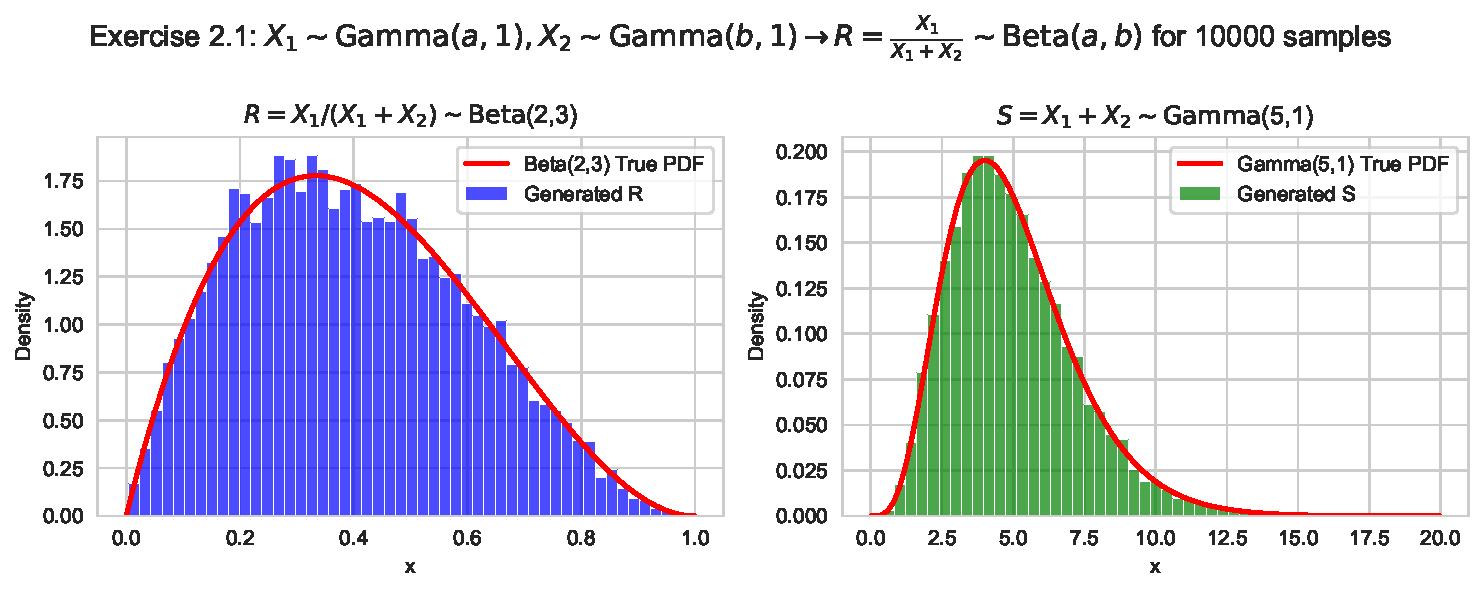
\includegraphics[width=0.9\textwidth]{exercise2_1.pdf}
\end{center}
\begin{center}
    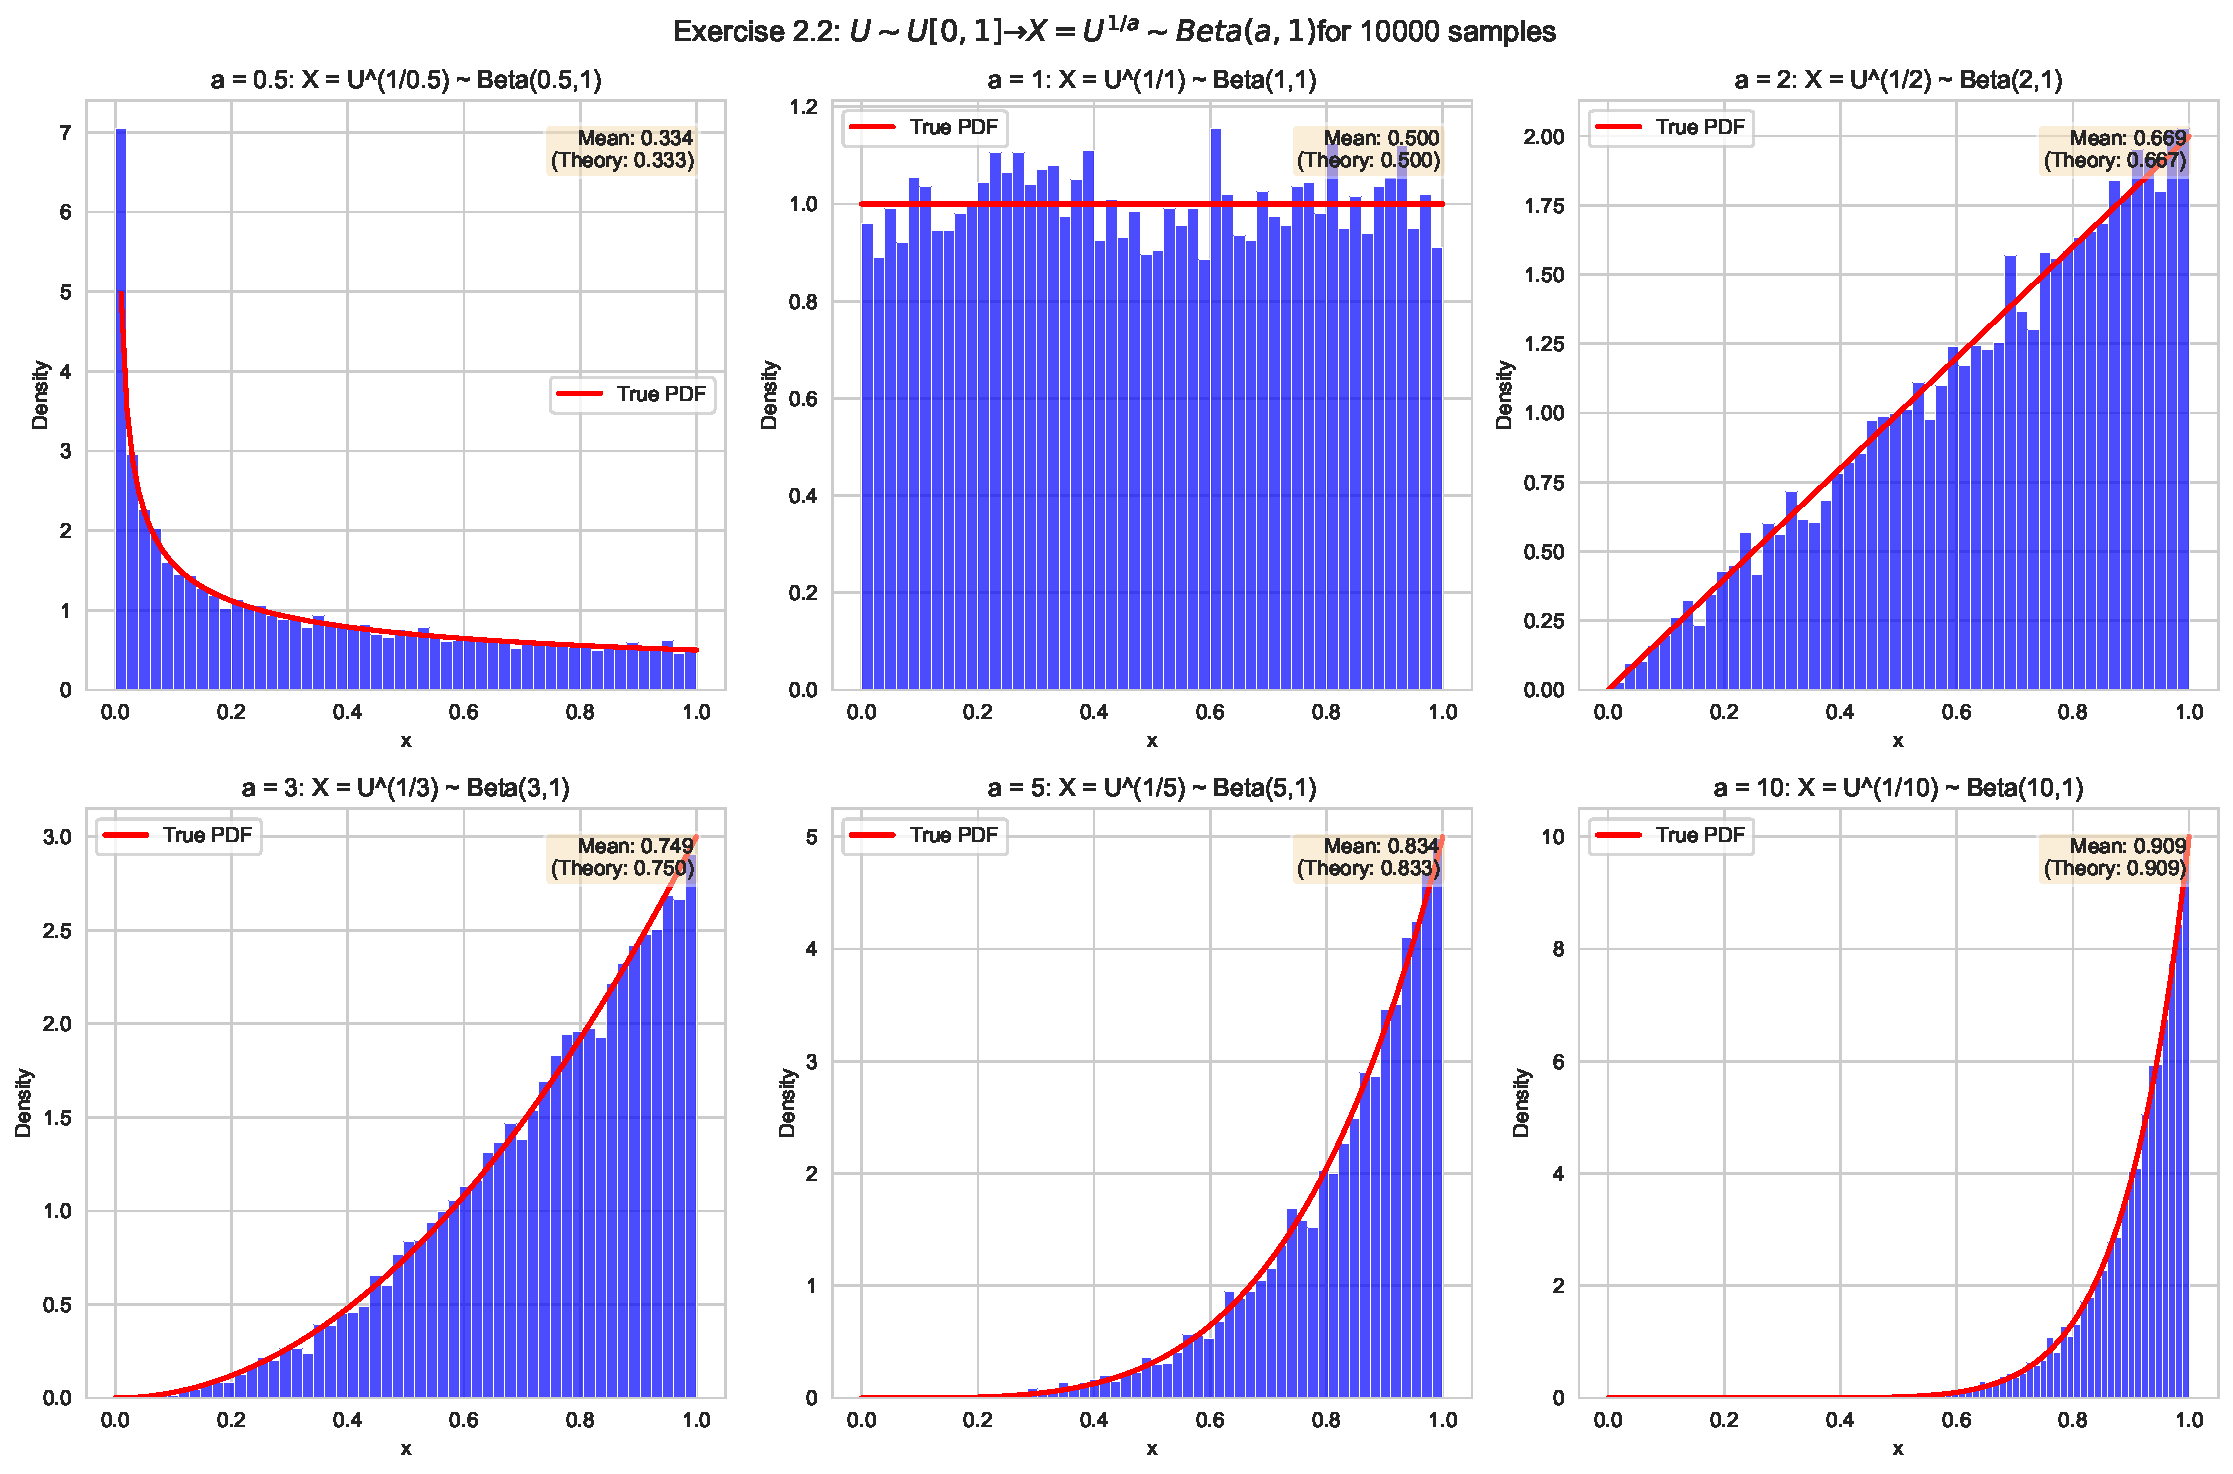
\includegraphics[width=0.9\textwidth]{exercise2_2.pdf}
\end{center}
\begin{center}
    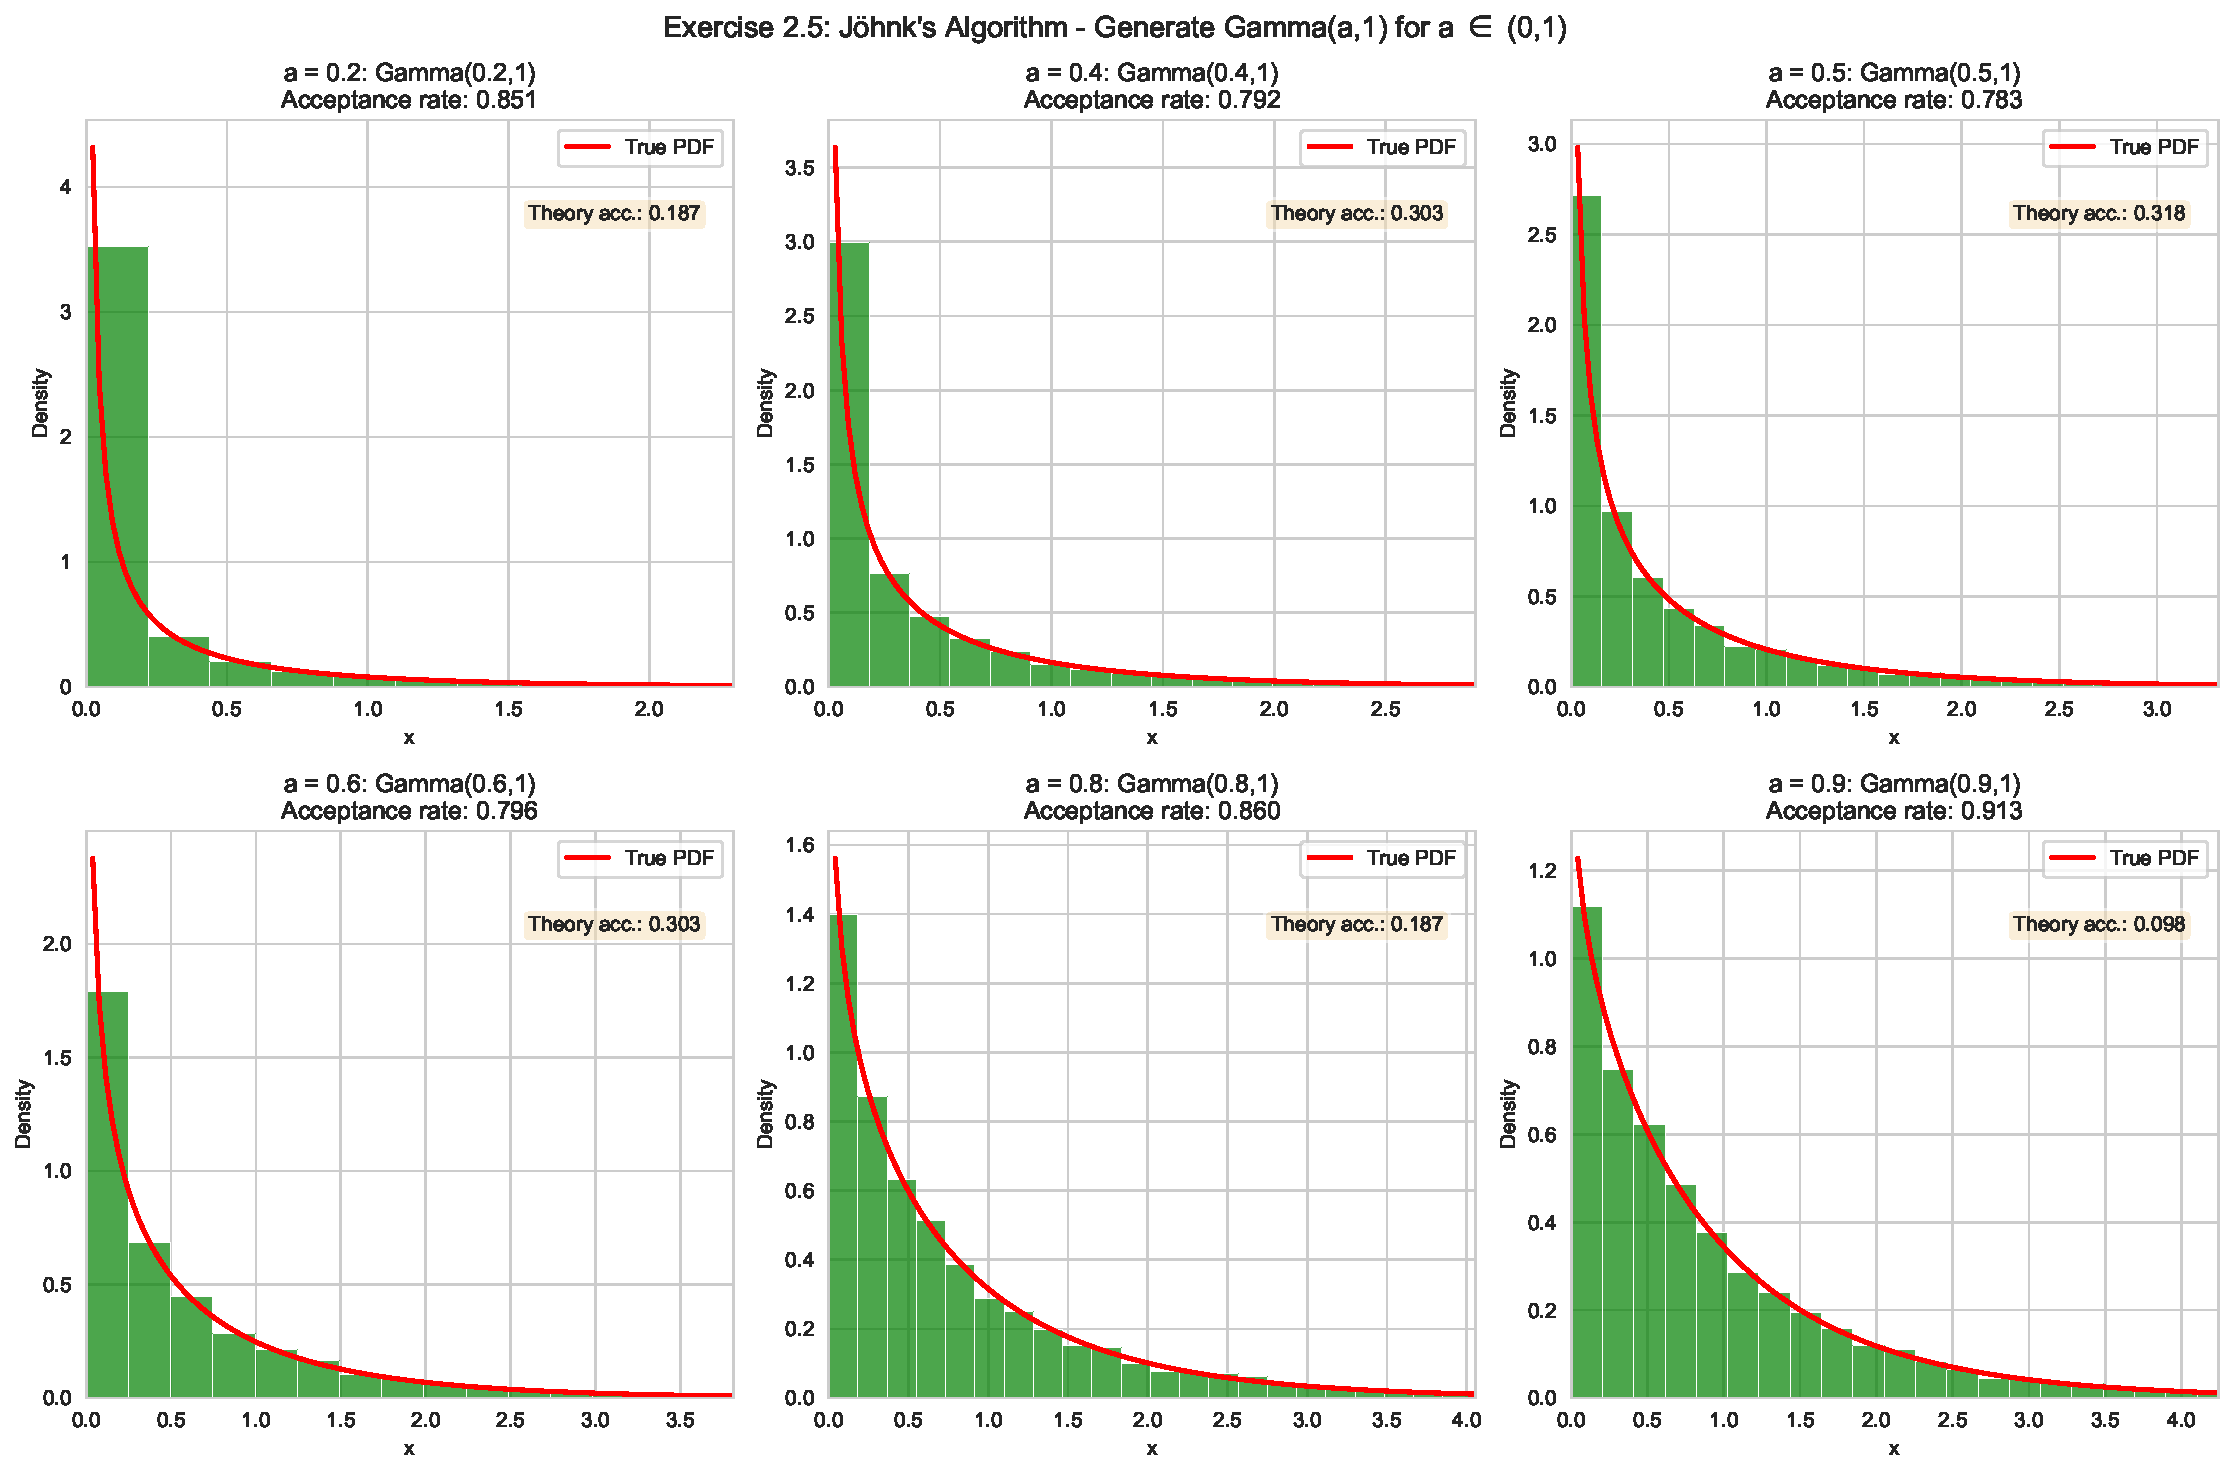
\includegraphics[width=0.9\textwidth]{exercise2_5.pdf}
\end{center}